\documentclass[aspectratio=169,11pt,english]{beamer}

% =========================================================
\usetheme{Berkeley}
\usecolortheme{default}

\definecolor{PythonBlue}{HTML}{306998}
\definecolor{PythonYellow}{HTML}{FFD43B}
\definecolor{DeepNavy}{HTML}{14213D}
\definecolor{SoftWhite}{HTML}{F7F9FC}
\definecolor{CodeGreen}{HTML}{2A9D8F}

\setbeamercolor{structure}{fg=PythonBlue}
\setbeamercolor{palette primary}{bg=DeepNavy,fg=white}
\setbeamercolor{palette secondary}{bg=PythonBlue,fg=white}
\setbeamercolor{palette tertiary}{bg=DeepNavy,fg=white}
\setbeamercolor{palette quaternary}{bg=PythonBlue,fg=white}
\setbeamercolor{title}{fg=white,bg=DeepNavy}
\setbeamercolor{frametitle}{fg=white,bg=DeepNavy}
\setbeamercolor{block title}{fg=white,bg=PythonBlue}
\setbeamercolor{block body}{fg=DeepNavy,bg=SoftWhite}
\setbeamercolor{alerted text}{fg=PythonBlue}
\setbeamercolor{normal text}{fg=DeepNavy,bg=white}
\setbeamercolor{item}{fg=PythonBlue}
\setbeamercolor{section in toc}{fg=PythonBlue}

\setbeamertemplate{navigation symbols}{}
\setbeamertemplate{items}[triangle]
\setbeamertemplate{blocks}[rounded][shadow=false]


\setbeamercovered{invisible}

% =========================================================
% PACKAGES
% =========================================================
\usepackage[T1]{fontenc}
\usepackage[utf8]{inputenc}
\usepackage{babel}
\usepackage{lmodern}
\usepackage{microtype}
\usepackage{graphicx}
\usepackage{booktabs}
\usepackage{mathtools}
\usepackage{amssymb}
\usepackage{xcolor}
\usepackage{listings}
\usepackage{tikz}
\usepackage{hyperref}
\usepackage{listings}
% =========================================================
% PYTHON CODE STYLE
% =========================================================
\lstdefinestyle{pythonstyle}{
	language=Python,
	basicstyle=\ttfamily\small,
	keywordstyle=\color{PythonBlue}\bfseries,
	stringstyle=\color{CodeGreen},
	commentstyle=\color{gray}\itshape,
	numbers=left,
	numberstyle=\tiny\color{gray},
	numbersep=8pt,
	showstringspaces=false,
	breaklines=true,
	frame=single,
	rulecolor=\color{PythonBlue!25},
	backgroundcolor=\color{SoftWhite},
	tabsize=4,
	keepspaces=true,
	columns=fullflexible
}
\lstset{style=pythonstyle}

% =========================================================
% metadata
% =========================================================
\title[CLASS 1.]{Introduction to Programming}
\subtitle{Python Fundamentals}
\author[ ]{Luis Ángel Bustos Ochoa}
\institute{Applied Physics}
\date{\today}

% =========================================================
% DOCUMENT
% =========================================================
\begin{document}
	
	% ---------------------------------------------------------
	% FRAME 1 — TITLE PAGE  ---------------------------------------------------------
{
	\setbeamercolor{background canvas}{bg=DeepNavy}
	\begin{frame}[plain]
		\centering
		\vspace{0.7cm}
		
		{\color{PythonYellow}\rule{0.22\textwidth}{2pt}}
		
		\vspace{0.65cm}
		
		{\color{white}\Huge\bfseries Introduction To Programming\par}
		
		\vspace{0.35cm}
		
		{\color{PythonYellow}\Large Python fundamentals\par}
		
		\vspace{0.8cm}
		
		\begin{tikzpicture}
			\node[
			rounded corners=8pt,
			fill=white,
			text=PythonBlue,
			inner sep=14pt
			] {
				\begin{minipage}{0.58\textwidth}
					\centering
					\ttfamily\Large
					Universidad...
				\end{minipage}
			};
		\end{tikzpicture}
		
		\vfill
		
		{\color{white}\large Luis Ángel Bustos Ochoa\par}
		\vspace{0.15cm}
		{\color{white!75}\normalsize Applied Physics \textbar{} Course: \par}
		
		\vspace{0.55cm}
		{\color{PythonYellow}\rule{0.22\textwidth}{2pt}}
		
		\vspace{0.35cm}
		{\color{white!70}\small\insertdate\par}
	\end{frame}
}	
	% =========================================================
	% SECCIÓN 1
	% =========================================================
	\section{Roadmap}
	
	% FRAME 2 — WHAT WE WILL LEARN TODAY
	\begin{frame}{Today...}
		\framesubtitle{Introduction to the course}
		
		{\large
			\begin{enumerate}
				\item Course info.
				\item Brief Introduction to a Computer Machine.
				\item Evolution
			\end{enumerate}
		}
	\end{frame}
	
	% =========================================================
	% SECCIÓN 2 =========================================================
	\section{Brief Introduction...}
		% FRAME 3 — THE IMPORTANCE OF TWO
	\begin{frame}{The importance of two}
		\framesubtitle{Brief Introduction to Information Theory}
		
		\begin{columns}[T] 
			
		
			\begin{column}{0.60\textwidth}
				\begin{itemize}
					\item We need at least two "cables" to complete a circuit.
					\pause
					\item We need a sender and a receiver to establish any form of conversation.
					\pause
					\item We only need two distinct states to describe and build a complete communication system.
				\end{itemize}
				
				\vspace{0.4em}
				\pause
				{\small The number 2 represents the fundamental minimum base for the existence and measurement of information.}
				
				\vspace{0.4em}
				\pause
				{\small \textbf{Therefore}, the number 2 is the absolute minimum required to build a complete "efficient" arithmetic system.}
			\end{column}
			
		
			\begin{column}{0.40\textwidth}
				\centering
				
			
				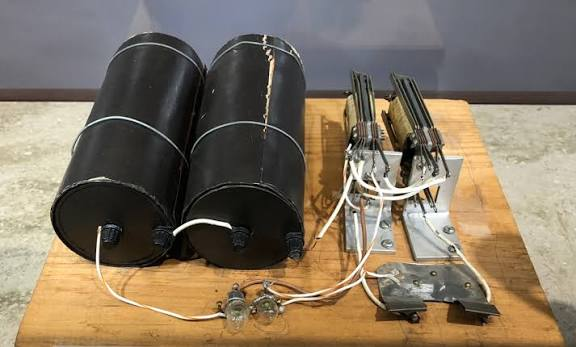
\includegraphics[width=0.85\textwidth,height=3.2cm,keepaspectratio]{model_k.jpg}
				\par
				{Stibitz's "Model K" (1937): Relays \& Batteries\par}
				
				\vspace{0.5em}
				
			
				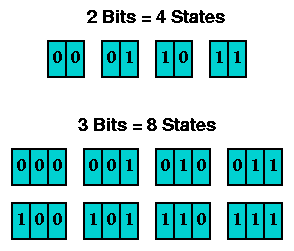
\includegraphics[width=0.85\textwidth,height=2.2cm,keepaspectratio]{binary_bits.png}
				\par
				{Two distinct states: 0 and 1 bits\par}
				
			\end{column}
			
		\end{columns}
	\end{frame}
	
	% =========================================================
% SECCIÓN 3: How Computers Wake Up
% =========================================================
\section{What does a machine do?}

% FRAME 4 — COMPUTER MACHINE: THE HARDWARE
\begin{frame}{Computer Machine}
	\framesubtitle{Powering on the system}
	
	\begin{columns}[T]
		% Left Column
		\begin{column}{0.55\textwidth}
			{\large \textbf{The Initial Spark:}}
			\vspace{0.5em}
			
			When you press the start button of your computer, a signal sends voltage across your hardware components. 
			
			\vspace{0.8em}
			This sudden flow of electricity synchronizes the subsystem, preparing the physical architecture to communicate with the software.
		\end{column}
		
		% Right column 
		\begin{column}{0.45\textwidth}
			\centering
			
			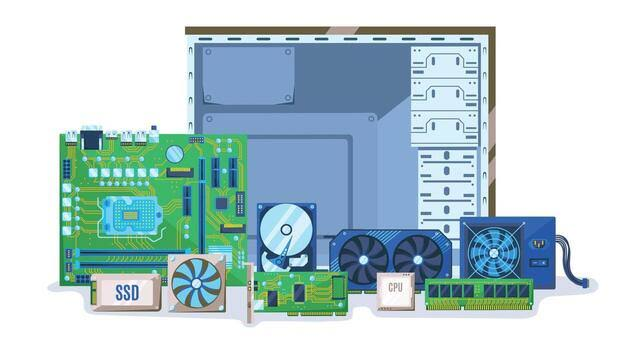
\includegraphics[width=\textwidth,height=5cm,keepaspectratio]{computer_parts.jpg}
			\par
			{Hardware Architecture \par}
		\end{column}
	\end{columns}
\end{frame}

% FRAME 5 — THE INTELLECT OF THE MACHINE: CPU & KERNEL
\begin{frame}{Inside the Brain}
	\framesubtitle{The CPU and the Kernel}
	
	\begin{columns}[T]
		% Columna Izquierda: El Procesamiento
		\begin{column}{0.55\textwidth}
			{\large \textbf{Executing the First Instructions:}}
			\vspace{0.5em}
			
			First, the CPU (Central Processing Unit) wakes up and "activates the kernel".
			
			\vspace{0.5em}
			\pause
			The kernel contains core instructions stored in memory, highly dependent on your Operating System.
			
			\vspace{0.5em}
			\pause
			The CPU executes \textbf{millions of operations per second} just to initialize the graphic system and show you the login screen.
		\end{column}
		
		% Columna Derecha: El CPU físico de cerca
		\begin{column}{0.45\textwidth}
			\centering
			
			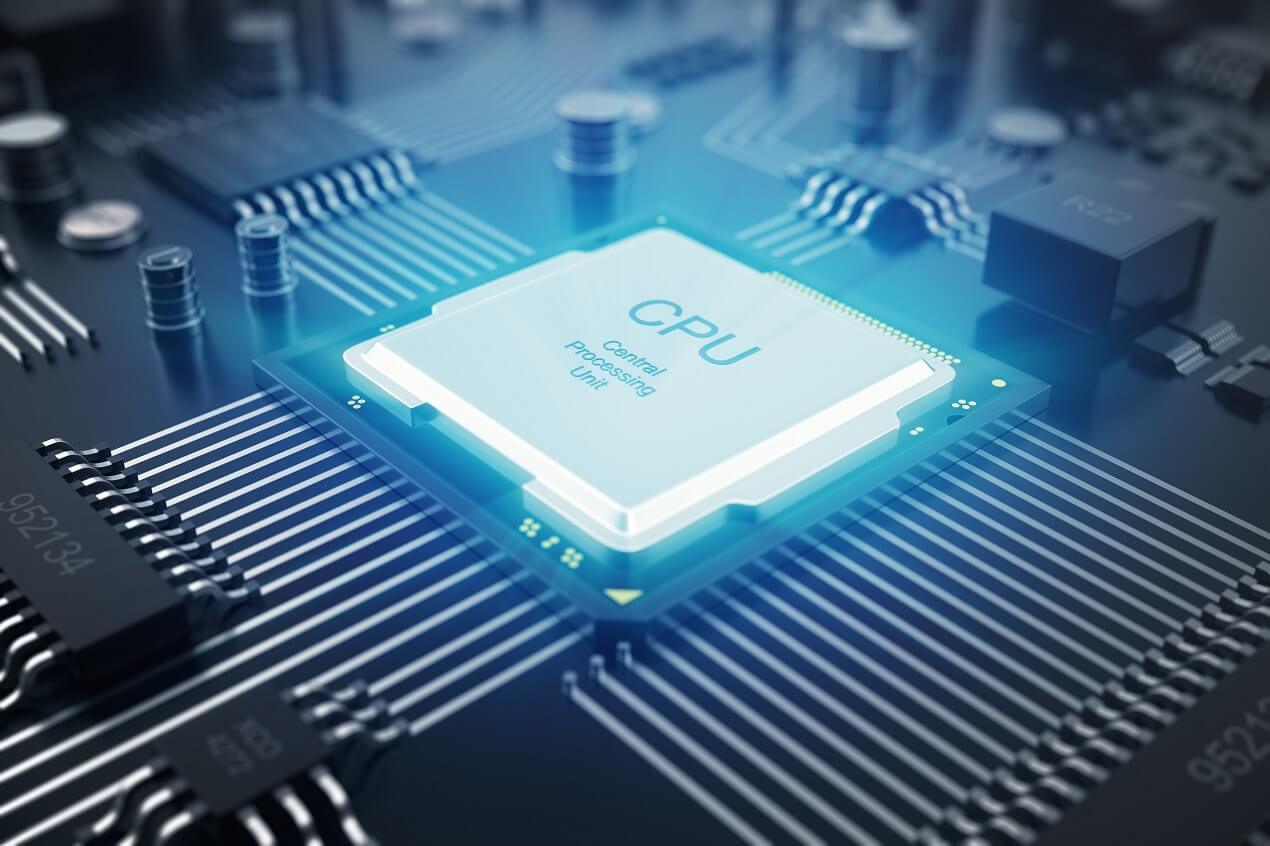
\includegraphics[width=0.95\textwidth,height=5cm,keepaspectratio]{cpu.jpeg}
			\par
			{Modern Central Processing Unit (CPU) \par}
		\end{column}
	\end{columns}
\end{frame}
\begin{frame}{The thinks that computers do:}
	\framesubtitle{calculate billions of simple operations per second and remember thinks}
		\centering

	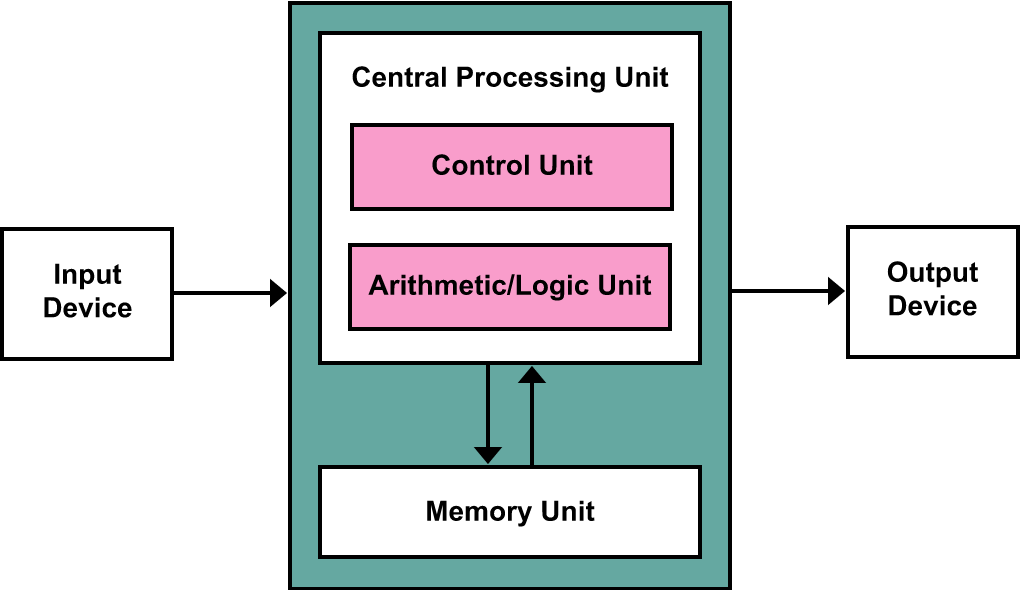
\includegraphics[width=0.99\textwidth,height=5cm,keepaspectratio]{basic_architecture.png}
	\par
	{ Basic Machine Architecture\par}
\end{frame}

% =========================================================
% SECCIÓN 4: Evolution of Languages
% =========================================================
\section{Evolution}

\begin{frame}{"The Eniac"}
	
	\begin{columns}[T]
	
		\begin{column}{0.48\textwidth}
%			\begin{block}{The Hardware (1945)}
%				\small First general-purpose electronic digital computer. Massive and complex.
%			\end{block}
			\vspace{0.5em}
			
		
			\centering
			\setlength{\unitlength}{1mm}
			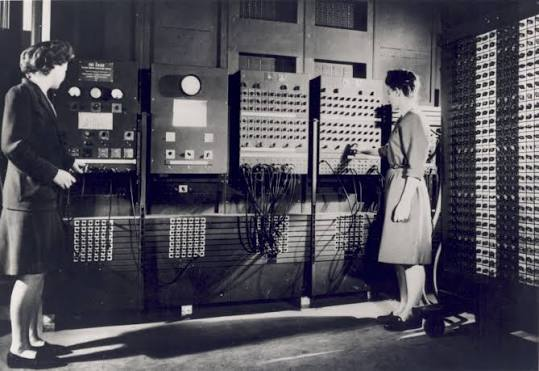
\includegraphics[width=0.99\textwidth,height=5cm,keepaspectratio]{eniac.jpeg}
			
			\vspace{0.5em}
			\centering
			{\color{black!90}{18,000 vacuum tubes, 30 tons.}}
		\end{column}
		
		
		\begin{column}{0.48\textwidth}
%			\begin{block}{The Logic (Boolean)}
%				\small At its core, everything relies on binary states controlled by electronic switches.
%			\end{block}
			\vspace{0.3em}
			\vspace{0.5em}
			
			
			\centering
			\setlength{\unitlength}{1mm}
			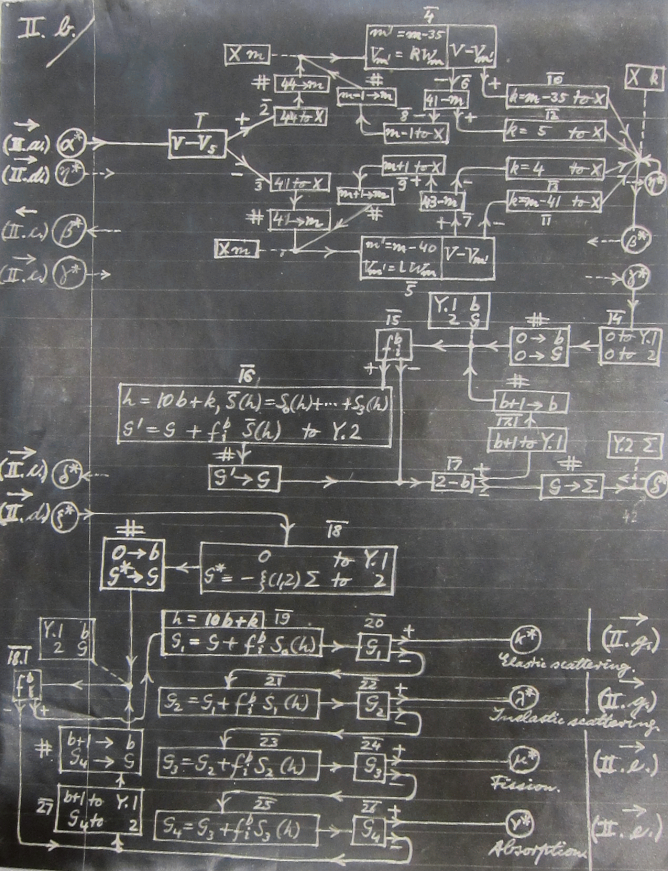
\includegraphics[width=0.99999\textwidth,height=4.3cm,keepaspectratio]{diagrama.png}
			
			\vspace{0.5em}
			\centering
			{\color{black!90}{Diagram of subroutines, nested loops for the Eniac.}}
%			\begin{lstlisting}[
%				language=Python, 
%				basicstyle=\ttfamily\footnotesize\color{black!80},
%				keywordstyle=\color{blue!80!black}\bfseries,
%				numbers=none,
%				frame=single
%				]
%				# Boolean Switch Logic
%				VacuumTube_1 = True  # ON (1)
%				VacuumTube_2 = False # OFF (0)
%				
%				# Logical AND gate inside ENIAC
%				Signal = VacuumTube_1 and VacuumTube_2
%				print(Signal) # Output: False
%			\end{lstlisting}
%			
%			\vspace{0.2em}
%			\centering
%			{\footnotesize\color{green!60!black}{$\rightarrow$ $1$ = Current, $0$ = No Current}}
		\end{column}
	\end{columns}
\end{frame}


\begin{frame}[fragile]{Nowadays...} 
	\begin{columns}[T] 
		% Columna IZQUIERDA: El Pasado (Bajo Nivel)
		\begin{column}{0.48\textwidth} 
			\begin{block}{Before: Low-Level (Assembly)} 
				\small Coding was about micro-managing the circuits and memory. 
			\end{block} 
			\vspace{0.3em} 
			\begin{lstlisting}[language={[x86masm]Assembler},basicstyle=\ttfamily\footnotesize\color{black!80},keywordstyle=\color{blue!80!black}\bfseries,commentstyle=\color{gray}\itshape,numbers=none,frame=none]
				MOV AX, 5 ; Initialize count 
				MOV BX, 3 ; Load modifier 
				ADD AX, BX ; Perform addition 
				PUSH AX ; Save result to RAM 
			\end{lstlisting} 
			\vspace{0.5em} 
			{\footnotesize\color{red!80!black}{$\rightarrow$ Hard to write, easy to break.}} 
		\end{column} 
		
		% Columna DERECHA: El Presente (Alto Nivel)
		\begin{column}{0.48\textwidth} 
			\begin{block}{Now: High-Level (Python)} 
				\small Coding is about solving logical problems in human-centric terms. 
			\end{block} 
			\vspace{0.3em} 
			\begin{lstlisting}[language=Python,basicstyle=\ttfamily\footnotesize\color{black!80},keywordstyle=\color{green!50!black}\bfseries,commentstyle=\color{gray}\itshape,numbers=none,frame=none]
				# Fully abstracted 
				total = 5 + 3 
			 	print(total) 
			 
			\end{lstlisting} 
			\vspace{0.5em} 
			{\footnotesize\color{green!60!black}{$\rightarrow$ Focus on logic, not hardware.}} 
		\end{column} 
	\end{columns} 
	
	\vspace{1.5em} 
	\centering \textbf{Evolution didn't make programming "easier"; it made it more powerful.} 
\end{frame}



\end{document}
